\section{Obecně}
Jak jsem již naznačil v předchozí kapitole, hybridní frameworky jsou nástroje, které umožňují vývojářům mobilních aplikací schovat svojí „webovou aplikaci“ do nativního obalu a na venkovní svět tak působit jako klasická nativní aplikace (více o tom, jak wrappery fungují si řekneme v Technickém popisu v podkapitole \ref{Sec:TechnickyPopis}).

\paragraph{Hlavní přednosti tohoto přístupu by se daly shrnout do několika bodů:}
\begin{enumerate}
        \item Přístup k nativním funkcím zařízení (fotoaparát, akcelerometr, výběr z kontaktů, geolokace apod.)
        \item Distribuce přes oficiální tržiště jednotlivých platforem
        \item Nezávislost aplikací na internetovém připojení
        \item Vývoj čistě pomocí webových technologií
        \item Podpora mnoha platforem (znovupoužitelnost velké části zdrojového kódu)
\end{enumerate}

"They are too cost effective and smart to ignore." Dominique Hazael-Massieux, lead of the Mobile Web Initiative at The W3C. \cite{bii_hybrid_apps_report}

Hybridní frameworky jsou tedy využívány pro vývoj mobilních aplikací, zejména pokud má vývojář v úmyslu zasáhnout více platforem ve velmi krátkém čase. Za tímto účelem mu zapouzdřovače poskytují adekvátní nástroje.

Je velice pravděpodobné, že do doby než formát HTML5 skutečně dozraje, budou hybridní postupy stále častější volbou webových vývojářů. Společnost Gartner předpovídá, že v roce 2016 bude víc než 50 \% všech mobilních aplikací hybridních. \cite{gartner_says_50}

"Increasingly, enterprises are finding that they need to support multiple platforms, especially as the [bring your own device] BYOD trend gains momentum."\cite{gartner_says_50}

Taková předpověď se samozřejmě neobjeví jen tak. Stojí za ní konkrétní problémy konkrétních firem, které musí řešit při budování strategie své firmy v digitální oblasti. Zákazníci od nich očekávají služby a aplikace určené přímo pro ně, pro jejich konkrétní platformu. Nesmělé pokusy velkého množství firem, které vyprodukují verzi 1.0 své aplikace pro jednu konkrétní platformu jsou typickým příkladem toho, kde se pro hybridní frameworky trh otvírá do široka.

I z toho důvodu se pozornost vývojářů otáčí k hybridním aplikacím. Gigant na poli enterprise řešení firma SAP v květnu loňského roku oznámila, že ve spolupráci s firmami Appcelerator (Appcelerator Titanium), Sencha (Sencha Touch) a Adobe (PhoneGap), bude svým zákazníkům v rámci svých širokých služeb nabízet i hybridní řešení. Součástí dohody je také poskytnutí možností k snadnému napojení zákaznických aplikací na data a služby, které SAP obvykle poskytuje \cite{bii_hybrid_apps_report}.

Právě problematika firemních aplikací je pro hybridní frameworky živnou půdou. Stále více totiž ve firemním prostředí sílí tzv. BOYD[a] přístup. BOYD je akronymem pro Bring Your Own Device. Tento přístup znamená, že zaměstnanci při práci používají své vlastní přístroje (notebook, mobilní telefon) a nenutí tak svého zaměstnavatele, aby jim je na své náklady poskytoval. Některé nové požadavky však na zaměstnavatele tento přístup přeci jen klade. Jde právě o začlenění těchto zařízení do chodu firemní sítě. Jedná se jak o příjem e-mailů, sdílených kalendářů apod., tak o přístup k firemním informačním systémům, kterých mohou být ve větších firmách desítky. Právě k tomu je vhodné mít širokou paletu mobilních aplikací, které budou umožňovat bezproblémové začlenění nových zaměstnanců do chodu společnosti, ať už používají jakýkoliv systém na kterékoliv platformě. Vývoj nativních aplikací pro tyto účely by však byl nákladově naprosto neúnosný. Bylo by nutné vyvinout všechny potřebné aplikace třeba ve 4-6 verzích, pro každou platformu zvlášť. To by si vyžádalo zaměstnání desítek draze placených vývojářů. A vzhledem k tomu, že se v drtivé většině nejedná o nijak graficky náročné aplikace, ale spíše o zobrazovače dat, použití hybridního přístupu se zde přímo nabízí. 

Pojďme si shrnout základní plusy a mínusy, které jsou s hybridním přístupem obvykle spojovány. Později se k nim ještě vrátíme.[b]

\begin{description}
        \item[+] Rychlejší „time to market“.
        \item[+] HTML5 vývojáři jsou obvykle levnější a snáze k sehnání.
        \item[+] Čím více HTML/CSS/JavaScript kódu, tím více ho můžeme znovupoužít pro port na jinou platformu.
        \item[+] Náklady na údržbu jsou obvykle nižší.
        \item[+] Délka schvalovacího procesu pro aktualizace je snížena na minimum.
        \item[-] Slabší výkon.
        \item[-] Hybridní frameworky a HTML5 stále nepokrývají všechny možnosti, které mají nativní vývojáři.
        \item[-] Apple se hybridním aplikacím brání a do budoucna je možno očekávat problémy při schvalovacím procesu.
\end{description}

Všechny výše uvedené argumenty je třeba zvážit ve chvíli, kdy se firma nebo vývojář rozhoduje, jakou technologii pro vývoj své aplikace použije. Pokud je aplikace spíše jednoduššího charakteru a neklade si vysoké nároky na grafický výkon, hybridní cesta bude pravděpodobně tou pravou. Naopak pro náročné hry a graficky sofistikované aplikace zůstává nativní přístup stále jedinou možností.

“The slickness of the user interface a developer can achieve in the native [app] model just isn’t worth the extra spending compared to the very nice level of user-interface experience they get from the hybrid option,” says Ron Perry, CTO of Worklight. \cite{hybrid_app_technology_overview}

\section{Technický popis} \label{Sec:TechnickyPopis}
Hybridní aplikace je složena ze tří zásadních komponent:

\begin{enumerate}
	\item Samotný kód aplikace napsaný zpravidla webovými jazyky HTML, CSS a JavaScriptem
	\item Webový runtime umožňující zobrazovat HTML a interpretovat JavaScript (UIWebView na iOS, WebView na Androidu)
	\item Tzv. „nativní most“, který zprostředkovává komunikaci mezi webovým runtimem (respektive samotnou aplikací) a operačním systémem.
\end{enumerate}

Strukturu hybridní aplikace naznačuje obrázek \ref{fig:HybridAppArchitecture}.

\begin{figure}\centering
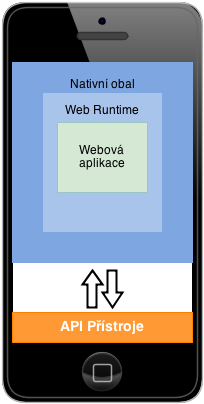
\includegraphics[width=0.4\textwidth]{hybrid_app_architecture.png}
\caption{Struktura hybridní aplikace \cite{ibm_worklight_overview}}
\label{fig:HybridAppArchitecture}
\end{figure} 

Pojďme si nyní detailněji popsat jednotlivé části. Samotná webová aplikace nemá zcela obvyklou strukturu, na kterou jsme zvyklí z tvorby klasických webových stránek. Velice často jde o jediný HTML soubor, kde je uvnitř elementu <body> ukryta celá architektura aplikace. Tento přístup umožňuje použití některého z oblíbených JavaScriptových frameworků, jako je např. jQuery Mobile, Zepto JS nebo Sencha Touch. Struktura samotné stránky pak vypadá nějak takto:


\begin{lstlisting}[language=HTML,breaklines=true]

<body>
<!-- Start of first page -->
<div data-role="page" id="foo">
  <div data-role="header">
    <h1>Foo</h1>
  </div><!-- /header -->

  <div data-role="content">
    <p>I'm first in the source order so I'm shown as the page.</p>
    <p>View internal page called <a href="#bar">bar</a></p>
  </div><!-- /content -->

  <div data-role="footer">
    <h4>Page Footer</h4>
  </div><!-- /footer -->
</div><!-- /page -->

<!-- Start of second page -->
<div data-role="page" id="bar">
  <div data-role="header">
    <h1>Bar</h1>
  </div><!-- /header -->

  <div data-role="content">
    <p>I'm the second in the source order so I'm hidden when the page loads.I'm just shown if a link that references my id is beeing clicked.</p>
    <p><a href="#foo">Back to foo</a></p>
  </div><!-- /content -->

  <div data-role="footer">
    <h4>Page Footer</h4>
  </div><!-- /footer -->
</div><!-- /page -->
</body>
\end{lstlisting}

Samotné přechody mezi stránkami jsou realizovány buď pomocí JavaScriptu funkcemi hide() a show() či využitím přechodů definovaných ve standardu CSS3. Výše zmíněné javascriptové frameworky většinou poskytují i CSS šablonu, ve které jsou definovány styly pro různé ovládací prvky, jakými jsou například tlačítka přívětivá pro dotyk. Vývojář si pak může tyto šablony přizpůsobit k obrazu svému přidáním vlastních pravidel.

Srdcem každé hybridní aplikace je však jeho javascriptový kód, ve kterém je definována celá aplikační logika. Pro její definování je často využíván právě framework jQuery, který zjednodušuje a urychluje používání některých oblíbených javascriptových funkcí. V JavaScriptu jsou definovány všechny reakce na události, uživatelské vstupy a výpočty na pozadí.

Abychom mohli HTML zobrazit uživateli, potřebujeme webový runtime, který bude umět náš kód zobrazit a průběžně vyhodnocovat. Většinou se jedná o osekané jádro webového prohlížeče, který je jinak v systému standardně přítomen. Právě v těch omezeních je však často skrytý zádrhel pro vývojáře. Například platforma iOS používá jako runtime UIWebView, jenž má narozdíl od mobilního prohlížeče Safari značnou nevýhodu v absenci javascriptového enginu Nitro, který je díky Just In Time kompilace velmi rychlý. V praxi to znamená, že pokud vaše hybridní aplikace používá JavaScript, bude UI [c]působit na uživatele pomaleji než identické UI spuštěné v prohlížeči Safari na tom samém zařízení. \cite{primer_on_hybrid_apps} Některé statistiky uvádějí, že javascriptový engine Nitro, který Safari používá, je více než 3x rychlejší než engine používaný v UIWebView. \cite{ios_for_html5_developer} Bohužel pro vývojáře není jiná možnost, jak toto omezení obejít, než používat co nejméně JavaScriptu je možné a pokoušet se ho nahradit například CSS3. Což je pro hybridní aplikace životně závisející na JavaScriptu velký problém.

Webový runtime není v podstatě ničím jiným než obyčejným objektem, který v sobě ukrývá renderovací jádro (např. WebKit). Původním smyslem tohoto objektu bylo dát možnost vykreslovat HTML obsah uživatelům v rámci nativních aplikací. Například Twitter ve své oficiální aplikaci používá takový webový runtime pro otevírání odkazů z tweetů. Uživateli se tak zobrazil obsah odkazu přímo v rámci aplikace a nemusel přepínat mezi aplikací a prohlížečem.

Tvůrcům hybridních frameworků se však podařilo uzpůsobit tyto objekty tak, aby se daly použít jako wrapper pro webovou aplikaci. Tohoto uzpůsobení je dosaženo pomocí rozšíření originálních tříd (UIWebView respektive WebView) v nativním kódu. Objekty jsou obohaceny o množství funkcí, které přispívají k optimálnímu běhu hybridní aplikace pomocí specifických reakcí na rozličné události.

Nyní, když chápeme jak funguje webový runtime, si můžeme vysvětlit jak probíhá komunikace mezi webovou aplikací a nativními funkcemi telefonu. Tato komunikace může probíhat v zásadě dvěma způsoby:

\begin{enumerate}
	\item Přímo z HTML pomocí HTML5 API.
	\item Pomocí volání konkrétních javascriptových funkcí dle specifikace konkrétního frameworku.
\end{enumerate}

Na prvním způsobu není nic zvláštního. V dnešní době jej mohou využívat i moderní webové stránky, pokud si je uživatel zobrazí v některém z novějších prohlížečů, jenž implementuje konkrétní funkci z HTML5 standardu. Všeobecně rozšířeným API voláním, které je možno volat přímo z HTML, je například geolokace nebo úložiště pro lokální ukládání dat. Tato volání vyhodnotí přímo webový runtime a sám se postará o zavolání konkrétní nativní funkce vhodné pro splnění požadavku.

\begin{figure}\centering
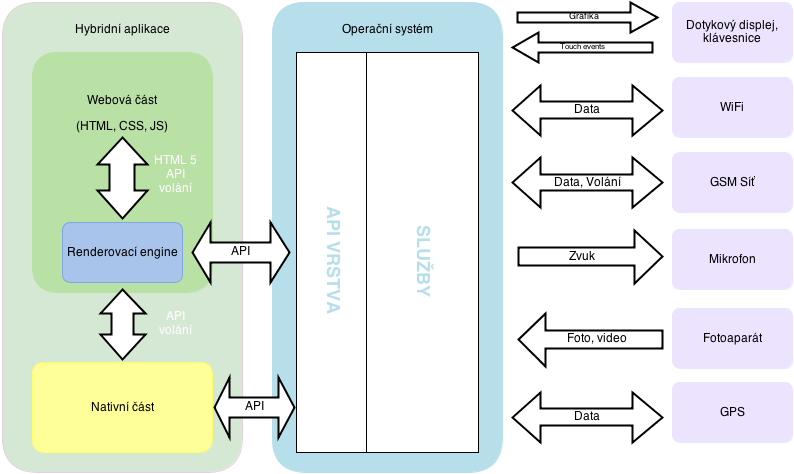
\includegraphics[width=1.0\textwidth]{hybridni_aplikace_komunikace.png}
\caption{Komunikace hybridní aplikace s operačním systémem}
\label{fig:HybridAppCommunication}
\end{figure} 

Větší pozornost si zaslouží druhý způsob komunikace s nativními funkcemi. Při něm již využijeme tzv. nativního mostu, který nám poskytuje samotný hybridní framework. Jedná se zpravidla o sadu tříd napsanou v nativním jazyce dané platformy, které slouží k zprostředkovávání komunikace mezi javascriptovými funkcemi definovanými v samotné webové aplikaci a operačním systémem zařízení, na kterém hybridní aplikace běží. V rámci každého operačního systému je třeba tento most implementovat odlišně. Každá platforma totiž umožňuje nějakým způsobem komunikovat mezi webovým runtimem a operačním systémem. Úkolem pro tvůrce hybridních frameworků je přijít s řešením, kterak zprostředkovat vývojáři sadu funkcí, které nezávisle na platformě poskytují aplikaci stejné služby a přitom nedat znát, že „za oponou“ probíhají zásadně odlišné procesy. Právě tato funkcionalita je klíčem k multiplatformnosti hybridních aplikací.

Logickým faktem je, že tzv. nativní most musí fungovat oboustranně, tj. nejen zpracovávat požadavky od webové aplikace, ale zároveň být schopen vrátit odpověď od operačního systému aplikaci zpět. Ač to zní jako poměrně triviální logika, každá z těchto cest je obvykle implementována velmi odlišně. Jak jsme již zmínil, implementace tohoto nativního mostu se může lišit framework od frameworku, já v rámci této sekce popíši, jak tento most funguje v nejpoužívanějším hybridním frameworku PhoneGap.

Ve PhoneGap je most mezi JavaScriptem a operačním systémem (v tomto případě Android) realizován pomocí Promptu. JavaScriptová API volání (například kamera, mikrofon apod.) jsou konvertována jako prompt příkaz, který je odposlechnut funkcí onJsPrompt definované webovým runtimem, která příkaz rozpozná a provede odpovídající nativní volání. \cite{dissecting_phonegap_architecture} 

Opačná cesta je realizována poněkud méně elegantním způsobem. Funguje na principu neustálého dotazování se nativní strany na odpověď. Aplikační strana se v intervalu 50 milisekund ptá nativní strany, zdali už je připravená odpověď na vznesený dotaz. Pokud je odpověď pozitivní, most zprostředkuje příchozí data klientské aplikaci.

V rámci operačního systému iOS vypadá schéma komunikace poněkud jednodušeji. V iOS funguje nativní most pro komunikaci směrem z klientské aplikace na principu iFrame, kdy jsou javascriptová volání nativních funkcí skladována ve frontě, ze které jsou následně čtena a prováděna pomocí nativní komponenty. Alternativou k tomuto přístupu je použití XHR dotazů. Klientská strana provede XHR dotaz na falešnou URL adresu v níž jsou umístěné příkazy, které se mají provést. Tyto příkazy jsou odposlechnuty, seřazeny a následně vykonány nativní stranou. \cite{dissecting_phonegap_architecture}

I komunikace opačným směrem je realizována poněkud jednodušeji, než je tomu u operačního systému Android. V iOS je veškerá zpětná komunikace prováděna pomocí funkce stringByEvaluatingJavaScriptFromString zprostředkované webovým runtimem UIWebView. \cite{dissecting_phonegap_architecture}

\section{Příklady hybridních frameworků}
\subsection{PhoneGap}
Vzhledem k tomu, že hybridnímu frameworku PhoneGap je věnována celá následující kapitola, zmíním ho zde opravdu jen velmi stručně.

PhoneGap je framework vlastněný a vyvíjený společností Adobe. Jedná se o zdaleka nejpopulárnější řešení na poli hybridních frameworků, což dokládá i fakt, že řada dalších hybridních frameworků na PhoneGapu staví a začleňuje jej do vlastních řešení.

PhoneGap v současné době oficiálně podporuje 7 mobilních platforem. V době psaní této bakalářské práce PhoneGap pokrýval 17 nativních API volání. Mezi ty nejpoužívanější dozajista patří geolokace, přístup k filesystému, fotoaparát či akcelerometr. Všechna API volání si podrobněji popíšeme v další kapitole spolu s detailním popisem celého frameworku PhoneGap.

\subsection{Sencha Touch}
Zařazení produktu Sencha Touch mezi hybridní frameworky je možná trochu odvážné. Já se toho přesto dopustím, protože Sencha Touch ve svých nejnovějších verzích poskytuje nástroje pro tvorbu hybridních aplikací, ač je jinak stále dominantně UI frameworkem.

Sencha Touch má za sebou již tři roky vývoje. Jejím primárním úkolem vždy bylo poskytovat vývojářům možnost rychle vyvíjet uživatelské rozhraní mobilních webových aplikací optimalizované pro použití na zařízeních s dotykovým displejem. Neméně důležité však je, aby zobrazované rozhraní vypadalo na dané platformě co možná nejvěrněji. V tomto přístupu se tedy příliš neliší od frameworku jQuery Mobile a dá se říci, že na poli javascriptových frameworků jsou právě jQuery Mobile a Sencha Touch těmi největšími konkurenty.

Hlavním posláním těchto UI frameworků je poskytnout vývojáři sadu vizuálních elementů jako jsou tlačítka, toolbary, seznamy, pop-up okna, formuláře, textová pole, přechody mezi stránkami atp., které mohou použít ve svých aplikacích, aniž by museli složitě pomocí CSS a JavaScriptu definovat tyto elementy sami. Zároveň jsou tyto vizuální prvky optimalizovány k maximální kompatibilitě a výkonu na co možná nejširším portfoliu webových prohlížečů.

Sencha v současné době podporuje 4 platformy (iOS, Android, Blackberry a Windows Phone 8). Použití tohoto produktu je pro většinu účelů zdarma, platit musíte jen pokud chcete na jeho základě postavit vlastní komerční framework.

Nyní si pojďme osvětlit, proč zařazuji Sencha Touch mezi hybridní frameworky. Vývojáři tohoto produktu totiž do jeho druhé verze přidali (v rámci nástroje Sencha Touch Preview SDK Tools) možnost přístupu k některým nativním API voláním mobilních platforem. Nabízejí také možnost zabalení webové aplikace do nativních binárních souborů vhodných k publikaci na oficiálních tržištích jednotlivých mobilních platforem. Sluší se dodat, že celá tato funkcionalita je stále značně omezená, protože podporovány jsou pouze dvě platformy (iOS a Android) a dostupné jsou pouze 4 API volání (indikace připojení k internetu, nativní notifikace, orientace zařízení a přístup k fotoaparátu). Dá se však očekávat, že se vývojáři pracující na frameworku Sencha Touch budou snažit dále rozšiřovat tento nástroj, aby podporoval více API volání a více platforem.

\subsection{MoSync Wormhole}
MoSync je velice zajímavý framework, který pokračuje de facto tam, kde PhoneGap končí. Nejedná se o klasický hybridní framework, neboť možnosti jeho využití jsou mnohem širší a hybridní funkcionalita do něj byla přidána až relativně nedávno.

Prapůvodním důvodem vzniku MoSync frameworku bylo umožnit vývojářům, kteří ovládají jazyky C nebo C++, vyvíjet nativní mobilní aplikace bez nutnosti měnit své programovací návyky a zároveň jim dát možnost zasáhnout více platforem najednou. Později byla přidána možnost vytvářet webové aplikace s využitím HTML5 a také hybridní aplikace s využitím obojího: HTML5 i nativního mostu napsaného v C/C++.

Vývojářům je tedy umožněno vytvářet klasické hybridní aplikace, ve kterých mohou přistupovat k nativním funkcím telefonu (geolokace, fotoaparát, filesystém apod.) a finální aplikace zabalit do nativních balíčků připravených na distribuci na oficiální tržiště. V současné době jsou pro hybridní účely podporovány tři hlavní platformy iOS, Android a Windows Phone[e].

\begin{figure}\centering
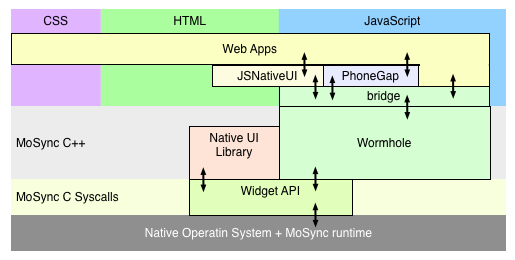
\includegraphics[width=1.0\textwidth]{MoSyncUI_Layers.png}
\caption{Architektura frameworku MoSync Wormhole \cite{javascript_for_native_widgets}}
\label{fig:MoSyncWormholeArchitecture}
\end{figure} 

Na obrázku \ref{fig:MoSyncWormholeArchitecture} můžeme vidět, jak funguje komunikace mezi webovou aplikací a nativním operačním systémem.

Celá tato hybridní technologie se nazývá Wormhole a její javascriptová část implementuje některé technologie z frameworku PhoneGap stejně jako některé novinky z HTML5 standardu (například geolokace). Velkou výhodou, kterou MoSync oproti PhoneGap nabízí, je možnost využít ve své aplikaci nativní UI elementy jako jsou tlačítka, různé lišty atp. To může být pro vývojáře skutečně zajímavé, protože bude využívat pravé nativní prvky místo často těžkopádných (v CSS emulovaných) náhražek. Tato technologie je však logicky úkrokem stranou od klasických wrapperů, které balí webové aplikace do webového runtimu. Jelikož webový runtime neumí vykreslovat nativní elementy, je pro tyto účely využit MoSync runtime, který pracuje s hybridní aplikací na podobném principu jako framework Titanium zmíněný ve třetí kapitole.

Fakt, že MoSync implementuje funkcionalitu z frameworku PhoneGap dodává tomuto nástroji další přidanou hodnotu. Většina aplikací napsaná ve PhoneGap je s MoSync kompatibilní a tak mohou vývojáři bezbolestně rozšířit své PhoneGap aplikace o nativní UI elementy, které poskytuje nástroj MoSync.

Framework MoSync je open-source a je šířen zdarma.

\subsection{IBM Worklight}
Worklight je vývojová platforma vyvíjená pod záštitou technologického giganta IBM. Umožňuje vývoj nativních, webových i hybridních aplikací. Tato platforma může být zajímavá zejména pro využití ve firmách, neboť pro enterprise účely přináší několik zajímavých nástrojů.

\paragraph{IBM Worklight umožňuje vyvíjet hybridní aplikace třemi způsoby \cite{ibm_worklight_overview}:}
\begin{enumerate}
	\item Vývoj klasické hybridní aplikace. Z vašeho javacriptového kódu voláte funkce operačního systému přes nativní most, který zajišťuje nástroj PhoneGap. Jedná se tedy o identický přístup, který používá většina hybridních frameworků.
	\item Vývoj částečně nativní aplikace. Vývojář může ve své aplikace využít zmenšeného web view a zbytek UI implementovat pomocí nativních UI komponent.
	\item Vývoj částečně hybridní aplikace. Uživatelé vyvíjejí kompletní uživatelské rozhraní pomocí nativních jazyků, ale pokud je to potřeba, mohou využívat i web views s hybridní funkcionalitou.
\end{enumerate}

IBM Worklight je celá sada nástrojů pro vývoj mobilních aplikací. Základem je IBM Worklight Studio – IDE postavené na open-source platformě Eclipse, které krom klasických funkcí nabízí i možnost tvorby uživatelského rozhraní pomocí WYSIWYG editoru. Vývojář si pomocí funkce drag \& drop přetahuje jednotlivé UI elementy (podporovány jsou HTML5, jQuery Mobile a Dojo Mobile) a modeluje si tím vzhled své aplikace.

Dalším užitečným nástrojem je IBM Worklight Server, který slouží jako middleware mezi uživatelskými aplikacemi a různými back-endovými systémy či cloudovými službami. Tato služba také řídí veškerý vzdálený přístup k aplikaci. Pro firemní účely dále obsahuje platforma Worklight nástroje jako jsou  IBM Worklight Application Centre, IBM Worklight Centre a IBM Worklight Device Runtime Components, které slouží ke vzdálené správě (přístup, push notifikace, analýza používání atd.) či distribuci (oficiální či privátní tržiště) aplikací.

\subsection{FeedHenry}
FeedHenry je společnost stojící za nástrojem Mobile Application Platform. Tato platforma je určena především pro enterprise segment trhu. Pro tvorbu hybridních aplikací je využíván PhoneGap, který zajišťuje propojení webové a nativní části.

Mobile Application Platform se zaměřuje především na pohodlné napojení aplikace na firemní back-end systémy a také na bezpečnost finálních aplikací, což jsou v korporátním prostředí vyhledávané benefity. FeedHenry dále poskytuje nástroje pro správu a analýzu aplikací v cloudu. Umožňuje jednoduché odeslání aplikací na privátní firemní tržiště, kde mohou firmy publikovat aplikace pro své zaměstnance či klienty.

\subsection{Icenium}
Icenium je, co se uživatelského přístupu týká, velmi inovativní nástroj. Veškerý vývoj totiž přesunul do cloudu. Nemusíte si stahovat žádné IDE či SDK. Pouze se zaregistrujete a vyvíjíte hybridní aplikace přímo v prohlížeči. Váš kód je umístěn buď ve verzovacím systému, který poskytuje samotný framework nebo můžete využít nástroje Git.

V cloudu se nachází i SDK jednotlivých platforem (v současnosti jsou podporovány pouze iOS a Android) a také knihovny nástroje Apache Cordova (PhoneGap), jehož služeb Icenium využívá. Krom vývojového prostředí se v cloudu nachází také testovací nástroje, které vývojářům umožňují real-time zobrazení uživatelského rozhraní a otestování funkčnosti samotné aplikace.

\subsection{WYSIWYG frameworky s využitím PhoneGap}
Do této skupiny řadím sobě podobné frameworky jako jsou například ApplicationCraft či Tiggzi, které vykazují společné znaky zejména v tom, že využívají pro tvorbu hybridních aplikací technologii z frameworku PhoneGap a zároveň jako primární způsob vývoje nabízí vývojářům v cloudu integrované WYSIWYG nástroje, kde je tvorba aplikací realizována pomocí mechanismu drag \& drop. Vývojář (nebo spíše modelář) aplikace skládá jednotlivé vizuální či funkční elementy a postupně tak vytváří svojí aplikaci. Díky využití PhoneGap může přistupovat k nativním funkcím operačního systému a následně hotovou aplikaci zabalit do nativního balíčku a distribuovat na oficiální tržiště.

\subsection{Srovnávací tabulka}
V následující tabulce naleznete přehledné porovnání jednotlivých hybridních frameworků dle následujících kritérií:

\begin{enumerate}
	\item Podporované platformy
	\item Podporovaná nativní API volání
	\item Poskytnutí vlastního IDE
	\item Licence a cena
\end{enumerate}

% TODO tabulka